\chapter{Risanje z voščenkami}
%
V članku \cite{DRudolf:BiWaxCrayon} predstavljeni postopek likovnega upodabljanja risanja z voščenkami modelira risanje na podlagi fizikalnih modelov, ki so bili eksperimentalno določeni in preizkušeni. Delu voščenke s katerim rišemo po papirju pravimo \emph{profil}. Voščenke so zgrajene iz mehkega in viskoznega materiala ter imajo standardni premer $8~mm$ (standardni večji premer meri $11~mm$). Zaradi velikosti profila pri stiku voščenke z risalnim papirjem ne smemo privzeti, da se profil spreminja homogeno na celotni površini, temveč moramo obravnavati spreminjanje profila na mikroravni. Pri risanju z voščenkami je pomemben začetni profil voščenke, ki vpliva na kasnejše spreminjanje profila, ko se material na profilu zaradi hrapavosti papirja neenakomerno kruši v plasteh.

Najprej bomo v prvem razdelku določili podrobnejše modele za voščenke in risalni papir, ki jih bomo uporabili v algoritmu. V drugem razdelku bomo predstavili ogrodje glavnega algoritma za likovno upodabljanje z voščenkami ter definirali potrebne pojme in (fizikalne) količine, ki jih bomo potrebovali. Pri eksperimentalnih poskusih je bilo opaženo, da pri risanju z voščenko na delu papirja, kjer je že bila nanešena plast voska, star nanos voska v smeri risanja potisnemo v sosednje območje, nekaj pa se ga lahko prime tudi nazaj na profil \ldots Ta opažanja bomo fizikalno opisali in predstavili algoritme za njihovo simulacijo. V naslednjem razdelku bomo s pomočjo KM barvnega modela, predstavljenega v \ref{chap:KMModel}, in eksperimentalno določenih parametrov za barve otroških voščenk predstavili končni algoritem, ki bo vrnil risbo narisano z voščenkami.

V zadnjem razdelku bomo opisali našo implementacijo algoritma in poskusno naredili slike z voščenkami, pri katerih uporabnik kot vhodni podatek ne bo podal skice v izbranih barvah za voščenke kot v članku, temveč bo podal (barvno) sliko, na podlagi katere bo program določil linije, ki jih bo pobarval z naračunanimi barvami voščenk.
%
\section{Model voščenke in papirja}
%
\subsection{Model voščenke}
%
Profil voščenke modeliramo kot dvodimenzionalno višinsko masko $M$, pri čemer vrednost posamezne celice $m_{i, j} \in M$ predstavlja pravokotno oddaljenost $h_{m_{i,j}}$ pripadajoče točke na profilu voščenke od \emph{osnovne ravnine} na kateri leži risalni papir. Maska $M$ mora biti dinamična, saj se pri risanju profil spreminja zaradi luščenja voska. Spreminjanje maske bomo opisali pri obravnavi algoritma.

Uporaba dinamične maske nam omogoča izbiro poljubnega začetnega profila voščenke. Za profile voščenk, pri katerih kot pravokotno projekcijo na osnovno ravnino dobimo krog, pravimo, da so \emph{okrogli profili}. Za slednje pravimo, da imajo \emph{polmer $R$}, kadar je premer voščenke enak $2\cdot R + 1$ (dodatna ena celica je tu iz tehničnih razlogov, saj pri implementaciji lažje operiramo z maskami lihe velikosti). Na sliki~\ref{fig:maske-voscenke} so prikazani nekateri možni profili, ki jih lahko uporabimo pri modeliranju risanja z voščenkami.

%
\begin{figure}[htbp]
  \centering
  \subfigure[]{
  
\includegraphics[width=0.2\textwidth]{./slike/wax}
  \ \ \ \ 
  \includegraphics[width=0.2\textwidth]{./slike/profil}
   }
   \ \ \ \ 
  \subfigure[]{
  
\includegraphics[width=0.2\textwidth]{./slike/waxp}
  \ \ \ \ 
  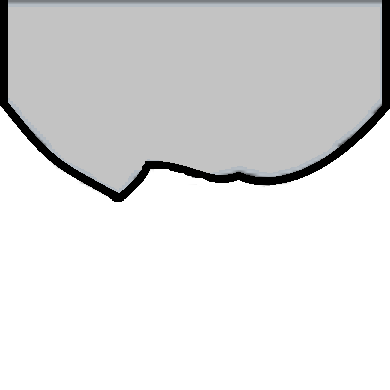
\includegraphics[width=0.2\textwidth]{./slike/profilp}
  }
  
  \subfigure[]{
  
\includegraphics[width=0.2\textwidth]{./slike/waxkot}
  \ \ \ \ 
  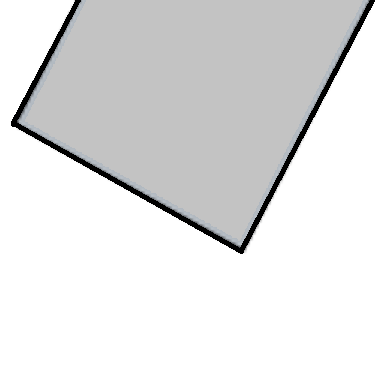
\includegraphics[width=0.2\textwidth]{./slike/profilkot}
  }
  \ \ \ \ 
  \subfigure[]{
  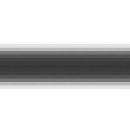
\includegraphics[width=0.2\textwidth]{./slike/waxl}
  \ \ \ \ 
  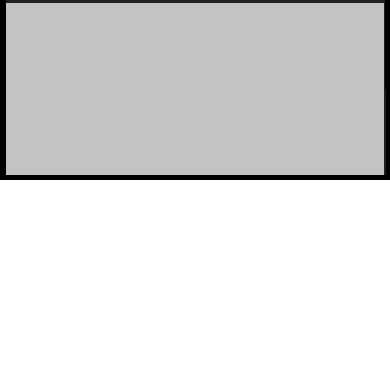
\includegraphics[width=0.2\textwidth]{./slike/profill}
  }
  \caption{Prikaz modelov za nekatere možne profile voščenke. Standardni profil voščenke je prikazan zgoraj levo. Intezitete slikovnih točk ustrezajo vrednostim $h_{m_{i,j}}$.}
  \label{fig:maske-voscenke}
\end{figure}
%

Celicam maske $M$ predpišemo tudi statično vrednost $u_{m_{i,j}}$, ki je sorazmerna deležu površine celice $m_{i,j}$, ki leži znotraj območja pravokotne projekcije profila na osnovno ravnino. Vrednost $u_{m_{i,j}}$ poimenujemo \emph{utež celice $m_{i,j}$}, za masko $M$ pa pravimo, da je \emph{utežena}. Z uporabo utežene maske se izognemu pojavu kvadratkastega videza končne slike (kar se pri dejanski izvedbi algoritma izkaže kot težava, še posebej pri uporabi profila voščenke na sliki \ref{fig:maske-profil3}, kadar voščenko nagnemo pod kotom manjšim od $20 \degree$). Na sliki \ref{fig:utezena-maska} je prikazan primer utežene maske okroglega profila voščenke s polmerom 6.

%
\begin{figure}[htbp]
  \centering
  \subfigure[]{
  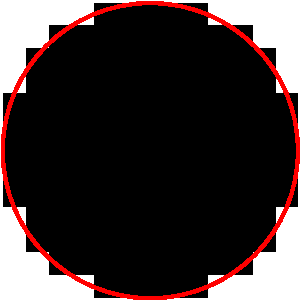
\includegraphics[width=0.2\textwidth]{./slike-latex/area.pdf}
  }
  \subfigure[]{
  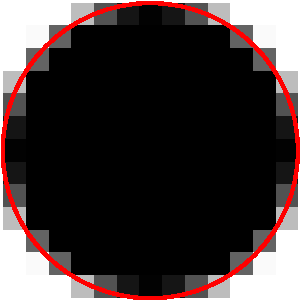
\includegraphics[width=0.2\textwidth]{./slike-latex/area-utez}
  }
  \caption{Prikaz modelov za nekatere možne profile voščenke. Standardni profil voščenke je prikazan zgoraj levo. Intezitete slikovnih točk ustrezajo vrednostim $h_{m_{i,j}}$.}
  \label{fig:maske-voscenke}
\end{figure}
%
\subsection{Model papirja}
%
\section{Modeliranje risanja z voščenkami}
%
Pri eksperimantalnih poskusih risanja z voščenkami opazimo, da se vosek s profila prenese na risalni list v neenakomernih plasteh in posledično spremeni obliko profila. Nadalje opazimo, da se vosek, ki je že nanešen na risalnem listu, če gremo ponovno preko njega z voščenko, prenese v sosednja lokalna območja v trenutni smeri risanja. Obravnava na mikroravni pokaže, da se prenese predvsem tisti del vosek, ki se nahaja na vrhih risalnega lista, in sicer v bližnje doline (glej siko \ref{fig:prenos-voska}). Prav tako pa se lahko manjša količina voska prime nazaj na profil.

%
\begin{figure}[htbp]
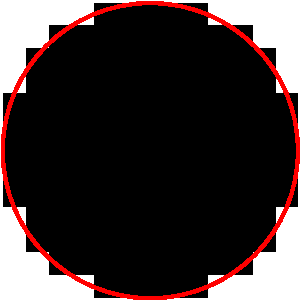
\includegraphics[width=0.2\textwidth]{./slike-latex/area.pdf}
\end{figure}
%
\subsection{Osnovne količine in algoritem za risanje posameznih linij}
%
Risanje posameznih linij simuliramo z algoritmom \ref{alg:glavniVoscenke}.

%
\begin{algorithm}[hbt]
  \caption{Povzetek glavnega algoritma za risanje z voščenkami.}
  \label{alg:glavniVoscenke}
\begin{algorithmic}[1]
\Require $P_1$, $P_2$, $M$, $C$, $f$, $L$
\Ensure Nova poteza z voščenko.
\Function {NovaLinija} {$P_1$, $P_2$, $M$, $C$, $f$, $L$}
  \For {$P_i \in \vec{P_1P_2}$} % TODO stavek \In
    \State \Call {PrilagodiVoščenko} {$P$, $M$, $f$, $L$}
    \State \Call {Redepozicija} {$P$, $\vec{V}$}
    \State \Call {Smearing} {$P_i$, $\vec{P_1P_2}$, $M$, $L$}
    \State \Call {DodajVosek} {$P_i$, $\vec{P_1P_2}$, $f$, $M$, $C$, $L$}
  \EndFor
\EndFunction
\end{algorithmic}
\end{algorithm}
%

Vhodni podatki algoritma so:
%
  \begin{itemize}
  \item $P_1, P_2$ $\ldots$ začetna in končna točka linije, ki jo bomo narisali,
  \item $M$ $\ldots$ maska profila voščenke,
  \item $C$ $\ldots$ barva voščenke,
  \item $f$ $\ldots$ velikost sile s katero pritiskamo voščenko na risalni list pri risanju,
  \item $L$ $\ldots$ seznamov posameznih nanosov voska (višina nanosa in njegova barva) za vsako slikovno točko na papirju.
  \end{itemize}
%
\subsection{Prilagoditev profila voščenke}
Na količino voska, ki se bo odluščil s profila, vplivajo naslednji dejavniki:
%
  \begin{itemize}
  \item površina profila,
  \item velikost in smer sile s katero pritiskamo voščenko pri risanju,
  \item relativna oddaljenost profila od risalnega lista,
  \item lokalna tekstura risalnega lista na trenutnem območju, kjer je profil voščenke.
  \end{itemize}
%
Pri risanju z voščenko se s profila lušči vosek, kar pomeni, da se veča skupna oddaljenost profila od ravnine risalnega papirja. Ker ohranjamo silo $f$ konstantno vzdolž ene linije, to pomeni, da bi na neki točki lahko izgubili stik med profilom in risalnim listom. Da se temu izognemu, bomo na vsakem koraku na novo prilagodili višino in obliko profila. Ob privzetku, da se dolžina voščenke zmanjšuje linearno, si bomo pri prilagajanju višine profila pomagali s Hookovim zakonom o kompresiji.
%
\subsubsection{Hookov zakon}
Hookov zakon lahko zapišemo v obliki
$$F = Y \frac{\Delta L}{L_0} A,$$
kjer so $Y$ Youngova konstanta modula, $\Delta L$ konstanta za stiskanje, $L_0$ nestisnjena dolžina voščenke in $A$ velikost profila. Ob privzetku, da je dolžina voščenke $L_0$ približno konstantna ($L_0 >> \Delta L$), lahko uvedemo novo konstanto $\lambda$, s katero se Hookov zakon prepiše v obliko:
%
\begin{equation}\label{eq:Hook2}
F = \lambda A \Delta L.
\end{equation}
%
Za konstanto $\lambda$ izberemo vrednost, ki nam bo dala estetsko primerne rezultate.
%
\subsubsection{Prilagoditev višine voščenke}
Kot smo že omenili, je zaradi velikosti površine profila, potrebna obravnava profila na mikroravni. V ta namen bomo po formuli \eqref{eq:Hook2} izračunali za vsako posamezno celico maske $m_{i,j} \in M$ prispevek k celotni sili: $F_{m_{i,j}} = \lambda \delta h$ ($A = 1$ za vsako celico profila). V primeru, ko med celico profila in istoležno točko na risalnem papirju ni stika (celica profila leži nad istoležno točko na risalnem listu), prispevek k sili nastavimo na 0. Skupna sila $F$ je enaka vsoti posameznih prispevkov, $F = \sum_{m_{i,j}} F_{m_{i,j}}$.

Količina $\delta h$ je v tem primeru razlika med višinama celice profila in istoležne točke na risalnem papirju skupaj z že nanešenim voskom. Višina celice profila bo tu odvisna od višine voščenke $h$, posledično je torej $F$ funkcija spremenljivke $h$, $F(h)$. Dobili smo aproksimacijski problem, pri katerem želimo čimbolje aproksimirati velikost sile $f$. Ker je $F$ vsota posameznih prispevkov, funkcija $F(h)$ ni več zvezna, lahko pa jo opišemo kot deloma zvezno funkcijo. Pri aproksimaciji si bomo pomagali z Newtonovo metodo. Natančnost aproksimacije in same simulacije pa nadziramo s konstanto napake $\varepsilon$. Eksperimentalno opazimo, da uporaba večje napake pohitri Newtonovo metodo, še vedno pa nam da likovno zadovoljive rezultate. V algoritmu \ref{alg:adjustCrayonHeight} je podana psevdokoda za določitev nove višine voščenke.

%
\begin{algorithm}[htb]
  \caption{Prilagoditev voščenke.}
  \label{alg:adjustCrayonHeight}
\begin{algorithmic}[1]
\Require $P$, $M$, $f$, $L$
\Ensure Spremenjena maska voščenke.
\Function {PrilagoditevVoščenke} {$P$, $M$, $f$, $L$}
  \State $h_{min}^{vo"s"cenka}$ $\gets$ $\displaystyle \min_{m_{ij} \in M} h_{m_{ij}}$
  \State $h_{min}$ $\gets$ $\displaystyle \min_{m_{ij} \in M} h_{P_{ij}}$ \Comment $P_{ij} = P + (i, j)$
  \State $h_{max}$ $\gets$ $\displaystyle \max_{m_{ij} \in M} h_{P_{ij}}$
  \While {$h_{max} - h_{min} > \Delta$}
    \State $h_{mid}$ $\gets$ $(h_{max} - h_{min})/2$
    \State $\getvalue{f_{mid}}{0}$
    \ForAll {$m_{ij} \in M$}
      \State $\delta h = h_{P_{ij}} + h_{L_{P_{ij}}} - (h_{m_{ij}} - h_{min}^{vo"s"cenka} + h_{mid})$
      \If {$\delta h > 0$}
        \State $\getvalue{f_{mid}}{\lambda \delta h}$
      \EndIf
      \If {$f < f_{mid}$}
        \State $\getvalue{h_{min}}{h_{mid}}$
      \Else
        \State $\getvalue{h_{max}}{h_{mid}}$
      \EndIf
    \EndFor
    \State $\getvalue{h_{mid}}{(h_{min} + h_{max})/2}$
    \ForAll {$h_{m_{ij}}$}
      \State $\getvalue{h_{m_{ij}}}{h_{m_{ij}} - h_{min}^{vo"s"cenka} + h_{mid}}$
    \EndFor
  \EndWhile
\EndFunction
\end{algorithmic}
\end{algorithm}
%

\subsection{Trenje}
Pri risanju z voščenko se bo zaradi mehkobe materiala iz katerega je zgrajena voščenka in trenja, ki nastane med voščenko in papirjem, vosek razporedil naokoli. %TODO a se reče mehkobe ali zakaj ...?
Trenje med voščenko in papirjem bomo opisali na makro in mikro ravni. Na makro ravni nas zanima normalna sila voščenke na površino papirja. Če voščenka preide mimo konveksnega % TODO konveksno za fizike
delčka v teksturi papirja, se bo od voščenke odstranil del voska, ki bo ostal za tem konveksnim delčkom papirja. Na mikro ravni uporabimo koeficient trenja, da aproksimiramo hrapavost papirja na manjši skali. Želimo, da je količina prestrukturiranega voska sorazmerna s silo trenja, ki je definirana kot
$$
\vec{F_F} = \mu \vec{F_N} = \mu \vec{N} \frac{\vec{N} \cdot \vec{F_C}}{\norm{\vec{N}} \norm{\vec{F_C}}}, %TODO wtf je s temi normami ???
$$
kjer je $\vec{F_C}$ sila voščenke na površino papirja, $\vec{F_F}$ je sila trenja, $\vec{F_N}$ je normala sile trenja na površino papirja, $\vec{N}$ je normala na površino papirja in $\mu$ je koeficient trenja papirja pri stiku z voščenko. % TODO ali se reče, da ima papir trenje, ali je trenje med papirjem in pa voščenko

Na podlagi teksture papirja interpoliramo sosednje vrednosti višin celic papirja, da dobimo ravnino po kateri se voščenka premika, in izračunamo silo trenja. Sila trenja je odvisna od naračunane ravnine, dane konstante sile trenja voščenke na papir in smeri risanja z voščenko.

Vrednost $\mu$ je odvisna od tega ali rišemo na čist papir ali pa je ta že porisan. Še več, območje papirja na katerem je debelina nanešenega voska voščenke večja, bo imelo drugačne lastnosti in trenje kot območja papirja s tanjšim slojem nanešenega voska voščenke. %TODO nanešenega ni v sskj ?
Če bi želeli biti rigorozni pri simulaciji trenja med voščenke in papirja, bi morali upoštevati zgornje. Vendar pa zaenkrat nimamo še rezultatov, ki bi povedali vrednost koeficienta za trenje papirja, ki bi dal rezultate kot bi jih želeli. Na področju teg bla bla \ref{24, 25} % TODO povej da mi bomo to kar malo tko naredli pa poglej še v članek nazaj; pa spiši neki
Pri naši simulaciji bomo določili posebej koeficient trenja za voščenko $\mu_{vo"s"cenka}$ in papir $\mu_{papir}$. Koeficient trenja bomo izračunali sproti kot linearno kombinacijo $\mu_{vo"s"cenka}$ in $\mu_{papir}$ na podlagi trenutnega faktorja.

V algoritmu \ref{alg:addNewWax} je podana psevdokoda za risanje z voščenko z upoštevanjem trenja.

%
\begin{algorithm}[htb]
  \caption{Risanje z voščenko in računanje trenja med voščenko in papirjem.}
  \label{alg:addNewWax}
\begin{algorithmic}[1]
\Require $P$, $\vec{V}$, $M$, $C$, $f$, $L$
\Ensure Dodan vosek. %TODO neki si zmisli, da bo tuki pisalo nekaj drugega kot izhodni podatki, ker to izhodni podatki v resnici niso
\Function {DodajVosek} {$P$, $\vec{V}$, $M$, $C$, $f$, $L$} % TODO neumno ime
  \State $\getvalue{\vec{V}}{\vec{V}/\max (x_{\vec{V}}, y_{\vec{V}})}$
  \ForAll {$m_{ij} \in M$}
      \State $\getvalue{P_{ij}}{P + (i, j)}$
      \State $\getvalue{\hat{P}_{ij}}{P_{ij} + \vec{V}}$
      \State $\getvalue{\vec{S}_{ij}}{(x_{\vec{V}}, y_{\vec{V}}, -h_{P_{ij}})}$
      \State $\getvalue{\vec{F}_{ij}}{(x_{\vec{V}}, y_{\vec{V}}, -f)}$
      \State $\getvalue{\vec{F}_{ij}}{1/(1 + h_{\hat{P}_{ij}}^{vo"s"cenka})}$
      \State $\getvalue{\mu_{ij}}{\alpha \mu_{papir} + (1 - \alpha) \mu_{vo"s"cenka}}$
      \State $\getvalue{\delta h_{\hat{P}_{ij}}^{vo"s"cenka})}{\mu (h_{\hat{P}_{ij}} - h_{m_{ij}}) \sin (\vec{S}_{ij}, \vec{F}_{ij})}$
      \State $\getvalue{h_{m_{ij}}}{h_{m_{ij}} + \delta h_{\hat{P}_{ij}}^{vo"s"cenka})}$ %TODO tile left{ right} se weird obnašajo - enormno veliki :(
      \State $\getvalue{L_{P_{ij}}}{L_{P_{ij}} + \set{(\delta h_{\hat{P}_{ij}}^{vo"s"cenka}), C)}}$
  \EndFor
\EndFunction
\end{algorithmic}
\end{algorithm}
%
%%
\section{Smearing}
Smearing je lastnost voščenke, podobno kot je krvavanje pri čopiču. % TODO krvavenje ni okej, neki drugega si zmisli
Pri risanju z voščenko na območjih z že nanešenim voskom voščenke, se vosek porazdeli in potisne bolj noter v luknje. % TDOo popravi to
Za simulacijo smeraringa bomo najprej uvedli smearing masko, ki upošteva trenutno točko in njene sosede. Vrednosti v maski voščenke določajo količino voska, ki se bo prenesel izpod trenutne točke in raznesel naokoli. Pri tem torej upoštevamo točko in njenih osem sosedov. Zaradi mehkobe materiala voščenke, predpostavimo,da je to dovolj upošteavti, medtem ko za nekatere druge materiale to ne bi bilo res (npr.\ pastelne barvice).
 
Pri simulaciji si bomo pomagali s filtrom $S$ velikosti $3 \times 3$. Elemente filtra izračunamo s formulo
$$S_{xy} = \frac{1}{\norm{(\vec{x, y})}} (\alpha \Delta z + \beta (\widehat{x, y}) \cdot \hat{V}).$$
Vrednost celice $S_{xy}$ nastavimo na 0, preprečimo morebitni prenos voska nazaj na voščenko. % TODO razmisli

V algoritmu \ref{alg:smearing} je podana psevdokoda za postopek smearinga.

%
\begin{algorithm}[htb]
  \caption{Smearing.}
  \label{alg:smearing}
\begin{algorithmic}[1]
\Require $P$, $\vec{V}$, $M$, $L$
\Ensure Posmearan papir.
\Function {Smearing} {$P$, $\vec{V}$, $M$, $L$} % TODO prevod
  \State $\getvalue{\vec{V}}{\vec{V}/\max (x_{\vec{V}}, y_{\vec{V}})}$
  \ForAll {$m_{ij} \in M$}
      \State $\getvalue{P_{ij}}{P + (i, j)}$
      \State $\getvalue{\hat{P}_{ij}}{P_{ij} + \vec{V}}$
      \State $\getvalue{\vec{S}_{ij}}{(x_{\vec{V}}, y_{\vec{V}}, -h_{P_{ij}})}$
      \State $\getvalue{\vec{F}_{ij}}{(x_{\vec{V}}, y_{\vec{V}}, -f)}$
      \State $\getvalue{\vec{F}_{ij}}{1/(1 + h_{\hat{P}_{ij}}^{vo"s"cenka})}$
      \State $\getvalue{\mu_{ij}}{\alpha \mu_{papir} + (1 - \alpha) \mu_{vo"s"cenka}}$
      \State $\getvalue{\delta h_{\hat{P}_{ij}}^{vo"s"cenka})}{\mu (h_{\hat{P}_{ij}} - h_{m_{ij}}) \sin (\vec{S}_{ij}, \vec{F}_{ij})}$
      \State $\getvalue{h_{m_{ij}}}{h_{m_{ij}} + \delta h_{\hat{P}_{ij}}^{vo"s"cenka})}$ %TODO tile left{ right} se weird obnašajo - enormno veliki :(
      \State $\getvalue{L_{P_{ij}}}{L_{P_{ij}} + \set{(\delta h_{\hat{P}_{ij}}^{vo"s"cenka}), C)}}$
  \EndFor
\EndFunction
\end{algorithmic}
\end{algorithm}
%
%%
\section{Redepozicija}
Ena izmed lastnosti voščenk je tudi ta, da se vosek, ko prečkamo območje, na katerem smo predhosno že nanesli plast voska, vosek nanese nazaj na voščenko. Pri premikanju voščenke po papirju se vosek, ki je že nanešen odkruši s papirja in lahko gre nazaj na voščenko ter se nato z voščenko prenese na drugo območje na papirju. Podoben problem je pri risanju s čopičem \ref{18, Baxter}. %TODO opis tega baxterja, neki je not v članku, mal bla bla

Zaradi viskoznosti materiala voščenke, se pigmenti v voščenki ne mešajo tako kot pri barvi, temveč se plasti voščenke odluščijo s papirja in pritisnjeo nazaj na voščenko. Ta vosek bo bil razporejen naokoli linearno in ne eksponentno. Barva s čopiča se prične mešati z barvo na platnu takoj ob stiku čopiča s platnom. Medtem, ko se pri voščenki nič voska ne bo razporedilo zgolj samo pri stiku.Z voščenko moramo podrgniti vosek iz papirja.

V algoritmu \ref{alg:reclaimWax} je povzeta psevdokoda za redepozicijo voska.

%
\begin{algorithm}[htb]
\caption{Redepozicija voska.}
\label{alg:reclaimWax}
\begin{algorithmic}[1]
\Require $P$, $\vec{V}$, $M$, $L$, $f$
\Ensure Razporejen vosek.
\Function {Redepozicija} {$P$, $\vec{V}$, $M$, $L$, $f$}
  \ForAll {$m_{ij} \in M$}
    \State $\getvalue {S} {3 \times 3 \text{ smearing mask}}$
      \ForAll {$s_{qr} \in S$}
        \State {$s_{qr}$} {$\max\set{0, \vec{V} \cdot \hat{(q, r)}}$}
      \EndFor
      \State $\getvalue {S} {\gamma f S / (\sum s_{qr})}$
      \State $\getvalue {\delta h_{vo"s"cenka}} {\max \set{0, h_{m_{i+q, j+r}} - h_{m_{ij}}}}$
      \State $\getvalue {L_{P_{ij}}'} {\set{l_a, \ldots, l_n} : \sum h_{l_i} \leq \delta h_{vo"s"cenka}}$
      \State $\getvalue {L_{P_{ij}}} {L_{P_{ij}} - L_{P_{ij}}'}$
      \ForAll {$s_{qr} \in S$}
        \ForAll {$l_k \in \delta L_{P_{ij}}'$}
          \State $\getvalue {m_{i+q, j+r}} {m_{i+q, j+r} + s_{qr} l_k}$
        \EndFor
      \EndFor
  \EndFor
\EndFunction
\end{algorithmic}
\end{algorithm}
% 
%%
\section{Upodabljanje z voščenkami}
Vosek je najlažje obravnavati kot prosojen pigment, za kar sta enostavna modela RGB in CMY pomankliva, da bi ju lahko uporabili. Namesto tega bomo uporabili Kubelka-Monk barvni model \ref{21}. KM model aproksimira spektralno prosojnost, sipanje in motnje. Vrednosti teh lastnosti lahko določimo s pomočjo dveh barv \ref{9}. Vsaka izmed teh barv je opaženi rezultat nanešene plasti na enobarvno ozadje (uporabimo belo in črno ozadje). Iz teh dveh barv KM model nato interpolira ti dve vrednosti, da dobi vrednosti za poljubne debeline nanešenega voska na ozadje katerekoli barve. KM model naredi to tako, da predvidi količino sipanja svetlobe glede na material pigmenta, in koliko je ta material prosojen. KM model aproksimira tudi spremembe, ki nastanjeo zaradi tankih motenj.

V našem modelu, ki ga bomo uporabili za risanje z voščenkami, bomo zanemarili motnje, saj v eksperimntalnih poskusih ni zaznati bistvenega vpliva. Posledično je vsaka voščenka predstavljena z enim naborom RGB barv ter parametrom prosojnost in sipanje.

Kot smo že omenili prej zelo tanke plasti voščenke združimo skupaj. Optične lastnosti končne plasti nastavimo na uteženo povprečje združenih plasti. Vsak prispevek plasti h končni plasti je torej sorazmeren z njegovo višino. To je groba peonostavitev KM modela, vendar še vedno da sprejemljive rezultate in bistveno zmanjša čas, ki je potreben za smearing.

Za upodobitev slike z voščenkami moramo vsaki točki na papirju $P_{ij}$ pripisati barvo $C_{P_{ij}}$. Za izračun barve, ki jo dobimo za plast $l_k \in L_{P_{ij}}$, uporabimo barvo plasti $C_{l_k}$, njeno prosojnost $t_{l_k}$ in sipanje $r_{l_k}$.

V algoritmu \ref{alg:render} je podana psevdokoda za upodabljanje slik z voščenkami.

%
\begin{algorithm}[htb]
\caption{Algoritem za upodabljanje slik z voščenkami.}
\label{alg:render}
\begin{algorithmic}[1]
\Require $T$
\Ensure Slika narisana z voščenkami.
\Function {Upodabljanje} {$T$}
  \ForAll {$P_{ij}$ teksture papirja $T$}
    \State $\getvalue {C_{ij}} {C_{P_{ij}}}$
    \ForAll {plasti voska $l_k$ v točki $P_{ij}$}
      \State $\getvalue {C_{ij}^{prosojnost}} {(t_{l_k} C_{l_k})^{h_{l_k}} C_{ij}}$
      \State $\getvalue {C_{ij}^{sipanje}} {1 - (1 - C_{l_k})^{r_{l_k} h_{l_k}}}$
      \State $\getvalue {C_{ij}} {C_{ij}^{prosojnost} + C_{ij}^{sipanje}}$
    \EndFor
  \EndFor
\EndFunction
\end{algorithmic}
\end{algorithm}
%
Eksperimentalno smo določili osnovne barve vočenk in njihove parametre. Podani so v tabeli \ref{tbl:voscenke}.

% TODO v novem članku so drugačne vrednosti !!!
\begin{table}[htb]
\begin{tabular}{ll|lll|ll}
\hline
Voščenka & Barva & R & G & B & t & s \\
\hline
& rdeča & 0.95 & 0.45 & 0.45 & 0.605 & 0.0425 \\
& oranžna & 0.999 & 0.55 & 0.3 & 0.77 & 0.03 \\
& rumena & 0.95 & 0.9 & 0.2 & 0.869 & 0.0425 \\
& zelena & 0.35 & 0.8 & 0.35 & 0.55 & 0.06 \\
& modra & 0.3 & 0.5 & 0.9 & 0.77 & 0.045 \\
& vijolična & 0.65 & 0.45 & 0.75 & 0.715 & 0.05 \\
& rjava & 0.8 & 0.6 & 0.55 & 0.495 & 0.075 \\
& črna & 0.26 & 0.25 & 0.245 & 0.935 & 0.05 \\
& siva & 0.42 & 0.4 & 0.39 & 0.594 & 0.275 \\
& bela & 0.8 & 0.8 & 0.78 & 0.88 & 0.175 \\
& periwinkle & 0.7 & 0.7 & 0.9 & 0.605 & 0.125 \\
& morsko zelena & 0.6 & 0.9 & 0.65 & 0.55 & 0.1 \\
& orhideja & 0.85 & 0.4 & 0.84 & 0.88 & 0.075 \\
\hline
\end{tabular}
\caption{Tabela z vrednostmi za barve, ki jih uporabljajo otroci (povzeto po članku \ref{voscenke}).}
\label{tbl:voscenke}
\end{table}
%